\chapter{Dizajn sustava}
\label{ch:system_design}

\selectlanguage{croatian}

\section{Arhitektura sustava}
\label{sec:architecture}

Predloženi sustav temelji se na modularnoj arhitekturi koja omogućuje fleksibilnost i 
proširivost. Sustav je podijeljen u nekoliko ključnih komponenti koje međusobno 
surađuju kako bi omogućile naprednu analizu meta podataka.

\begin{figure}[h]
    \centering
    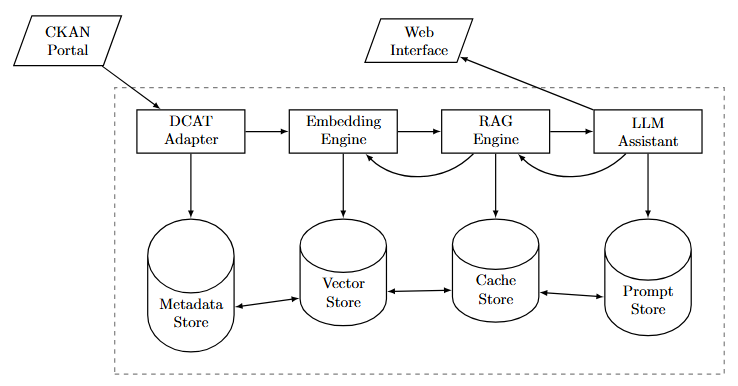
\includegraphics[width=0.8\textwidth]{figures/system_architecture}
    \caption{Arhitektura sustava za analizu meta podataka}
    \label{fig:system_architecture}
\end{figure}

\subsection{Ključne komponente}
Sustav se sastoji od sljedećih glavnih komponenti:

\begin{itemize}
    \item \textbf{DCAT Adapter} - komponenta za pretvorbu i normalizaciju meta podataka
    \item \textbf{Embedding Engine} - modul za vektorsku reprezentaciju meta podataka
    \item \textbf{Semantic Analyzer} - komponenta za semantičku analizu i otkrivanje veza
    \item \textbf{LLM Assistant} - sučelje za interakciju s korisnicima
    \item \textbf{CKAN Integration} - modul za integraciju s CKAN portalima
    \item \textbf{Web Interface} - korisničko sučelje sustava
\end{itemize}

\section{Prošireni DCAT model}
\label{sec:extended_dcat}

Za potrebe semantičke analize i povezivanja skupova podataka, razvijen je prošireni 
DCAT model koji dodaje nove funkcionalnosti standardnom DCAT modelu.

\begin{figure}[h]
    \centering
    \includegraphics[width=0.8\textwidth]{figures/extended_dcat_model}
    \caption{Prošireni DCAT model s podrškom za semantičke veze}
    \label{fig:extended_dcat_model}
\end{figure}

\subsection{Proširenja modela}
Ključna proširenja uključuju:

\begin{itemize}
    \item \textbf{Semantičke veze} - eksplicitno modeliranje veza između skupova podataka
    \item \textbf{Metrike kvalitete} - dodatni atributi za praćenje kvalitete meta podataka
    \item \textbf{Vektorske reprezentacije} - podrška za embeddings meta podataka
    \item \textbf{Kontekstualne informacije} - dodatni metapodaci o kontekstu i uporabi
\end{itemize}

\section{Tok podataka}
\label{sec:data_flow}

Tok podataka kroz sustav organiziran je u nekoliko faza koje osiguravaju učinkovitu 
obradu i analizu meta podataka.

\begin{figure}[h]
    \centering
    \includegraphics[width=0.8\textwidth]{figures/data_flow}
    \caption{Tok podataka kroz sustav}
    \label{fig:data_flow}
\end{figure}

\subsection{Faze obrade}
\begin{enumerate}
    \item \textbf{Dohvat podataka}
    \begin{itemize}
        \item Povezivanje s CKAN API-jem
        \item Dohvat meta podataka
        \item Validacija i normalizacija
    \end{itemize}
    
    \item \textbf{Semantička analiza}
    \begin{itemize}
        \item Generiranje embeddinga
        \item Analiza sličnosti
        \item Otkrivanje veza
    \end{itemize}
    
    \item \textbf{Obogaćivanje meta podataka}
    \begin{itemize}
        \item LLM analiza
        \item Generiranje opisa
        \item Dodavanje konteksta
    \end{itemize}
    
    \item \textbf{Pohrana i indeksiranje}
    \begin{itemize}
        \item Pohrana u vektorsku bazu
        \item Indeksiranje za pretraživanje
        \item Ažuriranje veza
    \end{itemize}
\end{enumerate}

\section{Korisničko sučelje}
\label{sec:user_interface}

Korisničko sučelje dizajnirano je s ciljem jednostavne i intuitivne interakcije s 
meta podacima i njihovom analizom.

\subsection{Komponente sučelja}
\begin{itemize}
    \item \textbf{Pretraživanje} - napredno semantičko pretraživanje
    \item \textbf{Vizualizacija} - grafički prikaz veza između skupova podataka
    \item \textbf{Interaktivni asistent} - sučelje za prirodnu jezičnu interakciju
    \item \textbf{Analitički dashboard} - pregled metrika i statistika
\end{itemize}

\section{Sigurnost i skalabilnost}
\label{sec:security_scalability}

\subsection{Sigurnosni aspekti}
Implementirane sigurnosne mjere uključuju:
\begin{itemize}
    \item Autentikacija i autorizacija
    \item Enkripcija podataka
    \item Praćenje pristupa
    \item Sigurnosno kopiranje
\end{itemize}

\subsection{Skalabilnost}
Sustav je dizajniran za skalabilnost kroz:
\begin{itemize}
    \item Modularnu arhitekturu
    \item Distribuiranu obradu
    \item Cachiranje rezultata
    \item Horizontalno skaliranje
\end{itemize}

\section{Integracija s postojećim sustavima}
\label{sec:integration}

\subsection{CKAN integracija}
Integracija s CKAN portalima ostvarena je kroz:
\begin{itemize}
    \item REST API adapter
    \item Sinkronizaciju meta podataka
    \item Mapiranje podatkovnih modela
    \item Praćenje promjena
\end{itemize}

\subsection{Proširivost}
Sustav podržava integraciju s drugim sustavima kroz:
\begin{itemize}
    \item Standardizirane API-je
    \item Prilagodljive adaptere
    \item Plugin arhitekturu
    \item Konfiguracijske opcije
\end{itemize} 